\documentclass{standalone}
\usepackage{tikz}
\usepackage{tkz-graph}
\usepackage{tkz-berge}

\begin{document}

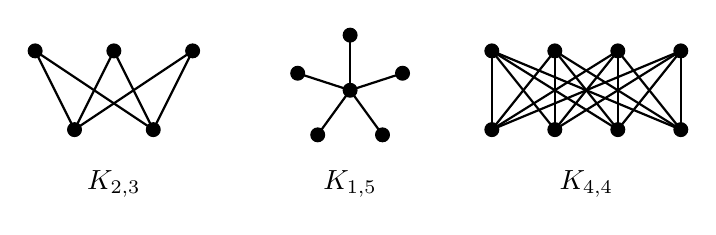
\begin{tikzpicture}
  \GraphInit[vstyle=Simple]
  \tikzset{VertexStyle/.style = {
  shape = circle,
  fill = black,
  inner sep = 0pt,
  outer sep = 0pt,
  minimum size = 5pt,
  draw}}
  \SetVertexMath
  \begin{scope}[yshift=2.2cm,xshift=-1cm]
    \grCompleteBipartite[RS=1.0,RA=1.0,RB=1.0]{2}{3}
  \end{scope}
  \begin{scope}[yshift=2.7cm, xshift=3cm, rotate=90]
    \grStar[RA=0.7]{6}
  \end{scope}
  \begin{scope}[yshift=2.2cm, xshift=4.8cm]
    \grCompleteBipartite[RS=1.0,RA=0.8,RB=0.8]{4}{4}
  \end{scope}
  \draw (0, 1.8) node [below]{$K_{2,3}$};
  \draw (3, 1.8) node [below]{$K_{1,5}$};
  \draw (6, 1.8) node [below]{$K_{4,4}$};
\end{tikzpicture}

\end{document}
